\documentclass[12pt]{article}
\usepackage{url}
\usepackage[spanish, english]{babel}
\selectlanguage{spanish}
\usepackage[fixlanguage]{babelbib}
\selectbiblanguage{spanish}
\usepackage{url}
\usepackage[utf8]{inputenc}
\usepackage{float}
\usepackage{fullpage}
\usepackage{amsmath}
\usepackage{amssymb}
\usepackage{graphicx}
\usepackage{verbatim} 
\usepackage{caption, subcaption}
\usepackage{tikz}%Generar plots
\usepackage{pgfplots}%Generar plots
\pgfplotsset{compat=1.5}
\usepackage{pgfplotstable,filecontents}
\usepackage{booktabs}
\usepackage{lipsum}

\pgfkeys{/pgf/number format/.cd,fixed,precision=5}

\usepackage[titletoc, title]{appendix}
\addto{\captionsspanish}{\renewcommand*{\appendixname}{Anexo}}

\bibliographystyle{bababbrv}

\title{Clasificación de Perros utilizando Bag of Words}
\author{Jorge Bahamonde, Sebastián González\\
\small{\url{jbahamon@ug.uchile.cl}, \url{segonzal@dcc.uchile.cl}}}
\date{}

\begin{document}
\maketitle

\section{Introducción}

La detección de animales en imágenes es una tarea compleja. La evolución ha llevado a
las criaturas a adaptarse a sus medios, siendo la mímesis con su entorno una de
las claves para la supervivencia de las especies; adicionalmente, los animales
domésticos han evolucionado al alero de la humanidad. En tiempos modernos, muchos animales viven en entornos urbanos,
y en su rol de mascotas son objetivo de retratos que son subidas a internet por sus dueños.

Presenta un problema adicional el que muchos de estos animales posean grandes diferencias entre sus razas: tamaño, color, textura, forma, etc.
El estudio de la detección de perros en un conjunto de imágenes es un problema
de interés, al ser un caso representativo de clasificación para una clase con características
altamente deformables. Por otro lado, una ventaja que brinda el estudio sobre
imágenes de perros es la alta disponibilidad de imágenes de prueba en internet:
los perros, siendo una de las mascotas más comunes, marcan una fuerte presencia en los retratos de mascotas.

En este trabajo se empleó la estrategia \emph{Bag of Words}, una de las técnicas en el reconocimiento de patrones que arroja mejores resultados para la clasificación.
Se puso énfasis en el estudio de esta estrategia para el reconocimiento de
imágenes de perros. En particular, se analizó el desempeño de la clasificación de SVM,
utilizando histogramas de palabras visuales, al variar la razón de costo asociado a los falsos positivos y falsos negativos ($\Theta$).

Se construyó un dataset de 1400 imágenes, de las cuales la mitad contienen
imágenes de perros extraidas del dataset Cats and Dogs.\cite{parkhi12a} Las
restantes imágenes no contienen perros y fueron extraidas aleatoriamente del
dataset caltech-101\cite{caltech101}. Por otro lado, se utilizó un \emph{corpus}
de 5000 imágenes del dataset caltech-256\cite{griffin2007caltech} para generar
las palabras visuales.

\section{Descripción del Trabajo}

Se estudió el desempeño de SVM sobre histogramas de palabras visuales, siguiendo la estrategia Bag of Words.

\subsection{Generación de palabras visuales}

Se definió un corpus formado por 5000 imágenes extraidas del dataset
caltech-256\cite{griffin2007caltech}. Para cada imagen se calcularon los
descriptores SIFT utilizando OpenCV.
Estos descriptores locales fueron clusterizados utilizando k-means, también a
través de OpenCV. Los $k$ centroides entregados por este método se utilizaron como
palabras visuales, para la posterior clasificación.

Se generaron palabras visuales para $k = 100, 500, 1000, 1500$.

\subsection{Entrenamiento}

Se utilizó la librería libSVM para la generación de los modelos. Los datos (es
decir, el valor de cada elemento de los histogramas que describen a cada imagen)
fueron escalados entre 0 y 1. Se utilizó validación cruzada para buscar los
mejores valores de $C$ y $\gamma$, los parámetros de entrenamiento. Cada modelo
utiliza histogramas de 100, 500, 1000 ó 1500 palabras visuales. Todos los
modelos fueron entrenados utilizando 500 imágenes del dataset generado y
utilizando el \emph{kernel} RBF.

\subsection{Clasificación}

Se clasificaron 400 imágenes, 200 de ellas conteniendo efectivamente perros,
utilizando los modelos entranados anteriormente. La salida de SVM es un par de
probabilidades $(\mathbb{P}_{dog},\mathbb{P}_{\neg dog})$.

Una imágen es clasificada como perro si:

\begin{equation}
    \frac{ \mathbb{P}_{dog} }{ \mathbb{P}_{\neg dog} } =
    \Theta
\end{equation}

Con $\Theta$ un umbral, el cual puede ser descrito como la función de costo de tener falsos positivos y negativos.

\subsection{Dataset utilizado}

Se construyó un dataset de 1400 imágenes en total. La mitad de estas imágenes
son imágenes de perros extraidas aleatoriamente del dataset Cats and Dogs\cite{parkhi12a}.  El
resto, 700 imágenes, no contienen perros, y fueron extraidas aleatoriamente del
dataset caltech-101\cite{caltech101}.  Se extrajeron 500 imágenes de perros y no-perros para
formar parte del set de entrenamiento.  Las 400 imágenes restantes forman el set
de prueba.

\section{Resultados obtenidos}

Para evaluar el desempeño del modelo estudiado, se le ultilizó para clasificar
imágenes entre dos clases: Perro y No-Perro. Se contrastaron los resultados
obtenidos con la clasificación correcta dada por la distribución en el dataset.

Se definen, en este contexto: 

\begin{itemize}
    \item el \textbf{número de positivos ($P$)} 200 imágenes en el set de prueba correspondientes a Perros.
    \item el \textbf{número de negativos ($N$)} 200 imágenes que no corresponden a Perros.
    \item el \textbf{número de falsos positivos ($FP$)} como el número de
        imágenes de prueba que el modelo identifica erroneamente como Perros.
    \item el \textbf{número de verdaderos positivos ($TP$)} como el número de
        imágenes de prueba identificadas correctamente como Perros.
    \item la \textbf{tasa de verdaderos positivos ($TPR$)} o probabilidad de detección correcta, es la razón $\frac{TP}{P}$;
    \item la \textbf{tasa de falsos positivos ($FPR$)} o probabilidad de detección incorrecta, es la razón $\frac{FP}{N}$.
\end{itemize}

De esta forma es posible estudiar el desempeño de este modelo de detección, comparando el comportamiento de ambas tasas.
El gráfico de $FPR$ versus $TPR$ al variar un tercer parámetro, en nuestro caso la función de costo $\Theta$, es denominado curva
ROC (del inglés \emph{receiver operating characteristic}).

Esta curva muestra
cuán apropiado puede ser un modelo o algoritmo para ciertas aplicaciones, ya que
el costo de un falso positivo versus un verdadero positivo varía dependiendo del
contexto.

\begin{figure}[h]
    \centering
   % \includegraphics{digit}

\begin{tikzpicture}
\begin{axis}[
        title={Curva ROC},
	xlabel={False Positive Rate},
	ylabel={True Positive Rate},
	grid=major,
	legend entries={$k=100$, $k=500$, $k=1000$, $k=1500$},
	legend style={at={(1,0)},anchor=south east},
]
\addplot table [scatter,x={FPR}, y={TPR}]{results100-ROC.csv};
\addplot table [scatter,x={FPR}, y={TPR}]{results500-ROC.csv};
\addplot table [scatter,x={FPR}, y={TPR}]{results1000-ROC.csv};
\addplot table [scatter,x={FPR}, y={TPR}]{results1500-ROC.csv};
\end{axis}
\end{tikzpicture}
    \caption{Curva ROC obtenida al variar el parámetro umbral $\Theta \in \{ 0.1,0.5,...,0.95\}$, para los cuatro modelos entrenados.}
\end{figure}

Se construyó una curva ROC a partir de los resultados de la clasificación con SVM comparando con su clasificación real conocida ya que es dada por su distribución en el dataset.

\section{Discusión}

En general se observan buenos resultados en la clasificación. Esta resulta mejor
para descriptores de $k=500$ y $k=1000$ palabras visuales.  Los falsos negativos
obtenidos (perros clasificados como no-perros) generalmente son imágenes en las
que el perro no juega un rol central: por ejemplo, cuando el fondo utiliza gran parte del
espacio de la imagen. Los falsos positivos obtenidos (no-perros clasificados
como perros) consisten en su mayoría en animales como gatos, canguros y rostros
humanos. Es probable que esta confusión se deba a la presencia de cabello, el
cual tiene palabras visuales comunes con el pelaje de los perros. Así,
complementar descriptores locales como SIFT con algún tipo de descriptor
orientado a la forma pudiera ayudar a mejorar este algoritmo.

De entre los modelos trabajados, el que utiliza 100 palabras visuales es el que
presenta el peor comportamiento. La baja cantidad de palabras visuales resultó,
en este caso, en que el modelo tiende a clasificar la mayoría de las imágenes
como perros, con lo que obtiene una alta tasa tanto de verdaderos positivos como
de falsos positivos.

\begin{figure}[H]
    \centering
    \subcaptionbox{No-Perro clasificado como Perro.}
{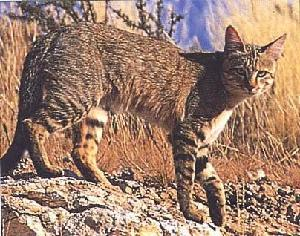
\includegraphics[scale=0.5]{../no-dogs/eval/96.jpg}
  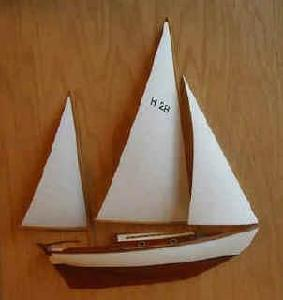
\includegraphics[scale=0.5]{../no-dogs/eval/157.jpg}}
    \subcaptionbox{Perro clasificado como No-Perro.}
{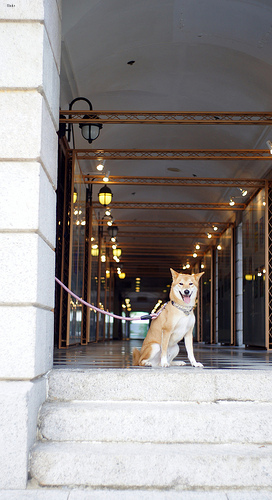
\includegraphics[scale=1.5]{../dogs/eval/122.jpg}
  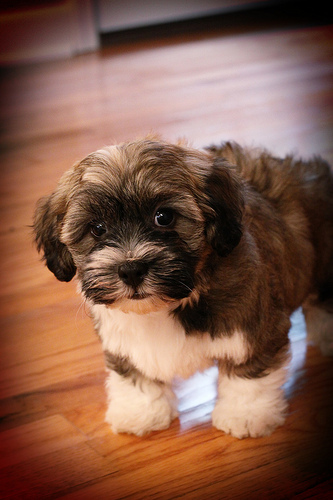
\includegraphics[scale=0.4]{../dogs/eval/194.jpg}}
    \caption{Errores de clasificación.}
\end{figure}

\section{Conclusiones}

A través de este trabajo se pudo apreciar cómo un método basado en descriptores
locales como SIFT puede ser utilizado para la clasificación de imágenes. Es
importante notar que aunque el método utilizado es relativamente genérico (por
ejemplo, no incluye intuiciones con respecto a las propiedades de los perros)
los resultados que entrega son bastante buenos. Se comprobó, además, cómo
bibliotecas como libSVM son capaces de facilitar el trabajo con modelos de
aprendizaje computacional relativamente complejos, permitiendo aplicar
estrategias como la validación cruzada para la elección de parámetros.

%bosquejando
El mejor desempeño de descriptores con un tamaño medio (dígase $k=500$ y
$k=1000$) tiene sentido. Descriptores con un gran vocabulario visual
posiblemente presenten conjuntos de palabras similares, sin un poder
discriminativo mayor que un vocabulario restringido. En el otro sentido, un
vocabulario muy pobre, no será suficiente para discriminar entre
características.

La estrategia Bag of Words responde bien frente a un set de datos heterogéneo.
Tiende a confundir animales con caracteristicas similares, con lo que usar un descriptor
de forma puede ayudar a filtrar los casos más extremos (como confundir un
perro con un rostro humano).  Para el caso de diferenciar animales muy similares
entre sí, como perros y gatos, el problema pudiera volverse mucho más complejo. 
%fin bosquejo

\selectlanguage{spanish}
\selectbiblanguage{spanish}

\bibliography{./informe}

\begin{appendices}

\section{Tasas de falsos positivos y verdaderos positivos obtenidas}

\begingroup
\centering
\pgfplotstabletypeset[col sep=tab,
%     columns={theta,FPR,TPR},
     display columns/0/.style={column name=$\Theta$},
     display columns/1/.style={column name=\emph{FalsePositiveRate}},
     display columns/2/.style={column name=\emph{TruePositiveRate}},
     every head row/.style={before row=\toprule,after row=\midrule},
     every last row/.style={after row=\bottomrule},
    ]{results100-ROC.csv}
\captionof{figure}{Tasas de falsos positivos y verdaderos positivos obtenidas.}\label{fig:f}
\endgroup


\end{appendices}


\end{document} 
